\clearpage
\section{Corrections}
This section describes several possible correction tools. All the functions are based on the pseudo-inversion using SVD (available in matlab) of an adequate Response Matrix (RM). 
All functions rely on orbit, trajectory and dispersion computations in 6D. Also BPM errors are always included in the simulations. The functions used for this purpose are: 
\begin{itemize}
\item \emph{findtrajectory6Err} : linepass starting at inCOD + BPM errors.
\item \emph{findorbit6Err} : orbit in 6D
\item \emph{finddispersion6Err} : moves RF frequency to observe orbit variation off energy
\end{itemize}

The functions implemented for correction (detailed below) are:
\begin{itemize}
\item \emph{atfirstturntrajectory} : correct first turn trajectory
\item \emph{atsetRFCavity} : correct RF frequency (uses RFCavityPass.c PassMethod)
\item \emph{atfittune,fittunedelta2fam} : correct tunes
\item \emph{atmatchchromdelta} : correct chromaticity
\item \emph{atcorrectorbit} : correct COD using steerers
\item \emph{atcorrectdispersion} : correct dispersion using quadrupoles
\item \emph{atdispersionfreesteering} : correct COD and dispersion using steerers
\item \emph{atRDTdispersioncorrection} : correct RDT and dispersion using quadrupoles
\end{itemize}
 
Also fitting functions can be implemented, but are often very dependent on the fit choices and on the available computing clusters. So they are not included here. 

\clearpage
\subsection{Response matrices}
All response matrices are computed by a common function that outputs the structure collecting the Responses that is used by all correction functions. The function \emph{getresponsematrices} centralizes the computation of all the matrices. A vector of integers is used to specify wich matrices to be computed and all functions have implemented a default RM computation calling \emph{getresponsematrices}. Below an example of call to \emph{getresponsematrices}.

\begin{lstlisting}
ModelRM...
        =getresponsematrices(...
        ring,...     % lattice to compute RM
        indBPM,...	 % Beam position Monitors indexes in ring
        indHorCor,...  % Horizontal steerers indexes in ring
        indVerCor,...  % Vertical steerers indexes in ring
        indSkewCor,...  % Skew quadrupole corrector indexes in ring
        indQuadCor,...  % Normal quadrupole corrector indexes in ring
        indSextCor,...  % Sextupole corrector indexes in ring
        [0 0 0 0 0 0]',...  % guess intial coordinated
        [1 2 3]);    % compute horizontal, vertical and dpp orbit response
\end{lstlisting}

The structure \emph{ModelRM} contains all the computed RM in different fields. All RM are normalized by the kick used for the computation and computed varying the relevant magnets on ``2 sides''. All oirbits are computed using 6D functions including BPM errors.

\begin{table}[hbp]
	\centering
		\begin{tabular}{l c r}
  index & response matrix computed & name of substructure \\
	\hline
	1  &   $\frac{\Delta  orbit (6D) }{ \Delta h steerer }$   &    ModelRM.OrbHCor \\
	\hline
  2  &    $\frac{\Delta  orbit (6D) }{ \Delta v steerer }$    &  ModelRM.OrbVCor \\
  \hline
  3  &    $\frac{\Delta  orbit (6D) }{ \Delta dpp       }$    &  ModelRM.OrbHDpp\\
     &    $\frac{\Delta  orbit (6D) }{ \Delta dpp       }$    &  ModelRM.OrbVDpp\\
  \hline
  4  &    $\frac{\Delta  trajectory (6D) }{ \Delta h steerer }$& ModelRM.TrajHCor\\
  \hline
  5  &    $\frac{\Delta  trajectory (6D) }{ \Delta v steerer }$& ModelRM.TrajVCor\\
  \hline
  6  &    $\frac{\Delta  trajectory (6D) }{ \Delta dpp       }$& ModelRM.TrajHDpp\\
     &    $\frac{\Delta  trajectory (6D) }{ \Delta dpp       }$& ModelRM.TrajVDpp\\
  \hline
  7  &    $\frac{\Delta  dispersion (6D) }{ \Delta h steerer }$& ModelRM.DispHCor\\
  \hline
  8  &    $\frac{\Delta  dispersion (6D) }{ \Delta v steerer }$& ModelRM.DispVCor\\
  \hline
  9  &    $\frac{\Delta  dispersion (6D) }{ \Delta dpp       }$& ModelRM.DispHDpp\\
  9  &    $\frac{\Delta  dispersion (6D) }{ \Delta dpp       }$& ModelRM.DispVDpp\\
 \hline
  10  &    $\frac{\Delta  dispersion (6D) }{ \Delta norm quad }$& ModelRM.DispQCor\\
 \hline
  11  &    $\frac{\Delta  dispersion (6D) }{ \Delta skew quad }$& ModelRM.DispSCor\\
 \hline
  12  &    $\frac{\Delta  tune            }{ \Delta norm quad }$& ModelRM.TuneQCor\\
	\hline
  	\end{tabular}
\end{table}


\clearpage
\subsection{Tune}
Tune is set using \emph{atfittune}. In case of large tune deviations affecting also the integer part, \emph{atmatchtunedelta} matches the total phase advance of the lattice to be corrected. 

\begin{lstlisting}
% atfittune
NEWRING = ATFITTUNE(RING,NEWTUNES,QUADFAMILY1,QUADFAMILY2);
\end{lstlisting}

\clearpage
\subsection{Chromaticity}
Since in a lattice with errors all sextupoles might have different strengths, the chromaticity correction is computed adding a common variation to 2 families of sextupoles. This is implemented using \emph{atmatch} in the function \emph{atmatchchromdelta}. Below an example. 

\begin{lstlisting} 
% sextupole indexes
indS=find(atgetcells(r0,'Class','Sextupole'))';
pbsxt=atgetfieldvalues(r0,indS,'PolynomB',{1,3});
indSF=indS(pbsxt>0);
indSD=indS(pbsxt<0);

% fit chromaticity adding a common variation to 2 sext failies             
rerr=atmatchchromdelta(rerr,chrom,{indSF,indSD});
\end{lstlisting}

\clearpage
\subsection{RF cavity}

The functions \emph{atsetRFCavity}is used to set the RF cavity frequency and time lag to the optimal values in presence of radiation and eventual lattice errors. Due to the available integration methods in AT (CavityPass and RFCavityPass), at the moment it is not possible to consider the true lattice elongation: in the cavity pass methods in AT the sum of the Length fields in all elements is considered as the length of the lattice. 

The function \emph{atRFcorrection} is used to set a zero average energy deviation in the lattice, by minimization of the COD using an RF frequency shift ( cancel dispersive contribution in the orbit). The time lag is the set according to the 6th coordinate in tracking at the cavities.

\begin{lstlisting}
% RF cavity parameters
rfv=9.0e6; % Volts
harm=992; 
radon= 1; % 1 = radiation on
DeltaHz=0; % no errors, frequency has no modification due to COD
           % this DeltaHz can be also used to see dispersive orbits.
					
% set RF cavity freqeuncy and time lag
[rerr]=atsetRFCavity(rerr,rfv,radon,harm,DeltaHz);

% correct RF frequency for <dpp>=0
[   rcor,...				%output corrected lattice
    inCODcor,...    % intial coordinate guess after correction
    fc....          % corrected RF frequency
    ]=atRFcorrection(...
    rerr,...        % lattice to be corrected
    indBPM,...      % BPM indexes for orbit computation
    inCOD,...       % initial orbit guess
    [1 1 1 1 1],... % number of eigenvectors for reiteration
    1,...					  % scaling factor for correction
    ModelRM,...     % response matrix, if [] will be computed
    zeros(2,length(indBPM)),... % reference orbit for correction
    true);          % verbosity flag

\end{lstlisting}

The correction of RF frequency for minimal energy deviation is not optimized for dynamic apertures, while the frequency obtained using \emph{atsetRFCavity} is always the best possible frequency.

\clearpage
\subsection{Orbit}

Orbit correction is performed using \emph{atcorrectorbit}. The functions implements several features for  correction:
\begin{itemize}
\item the average steerers strenghts 0, 
\item iteration of the correction varying the number of eigenvectors 
\item correction of the frequency (as in \emph{atRFcorrection}).
\item possibility to limit the steerers strengths
\end{itemize}

Below an example of usage of the orbit correction function. 
\begin{lstlisting}
[rcor,...           % corrected lattice
    inCOD,....      % initial orbit guess after correction
    hs,...          % total horizontal steerers strenghts
    vs....          % total vertical steerers strengths
    ]=atcorrectorbit(....
    rerr,...        % lattice to be corrected
    indBPM,...      % BPM indexes
    indHCor,...     % horizontal steerers indexes
    indVCor,...     % vertical steerers indexes
    inCOD,...       % input 6D closed orbit guess
    [...            % several correction iterations 
    [10 20];...     % with different number of eigenvectors 
    [30 40];...     % for horizontal and vertical plane
    [50 60];...     % <-- iter 3, use 50 eig hor., 60 eig ver.
    [70 70];...     % <-- iter 4, use 70 eig hor., 70 eig ver.
    [80 80];...     % <-- iter 5, use 80 eig hor., 80 eig ver.
    [97 96];...
    [97 96]...
    ],...
    [true true],... % [do dpp correction, keep average of correctors zero] 
    1.0,...         % scale factor for correction
    ModelRM,...     % response matrix, if [], compute it 
    zeros(2,length(indBPM)),... % reference orbit to correct to
    [0.5e-3 0.5e-3],... % sterrer strengths limits
    true);          % verbosity flag
\end{lstlisting}


\begin{figure}[!h]
	\centering
	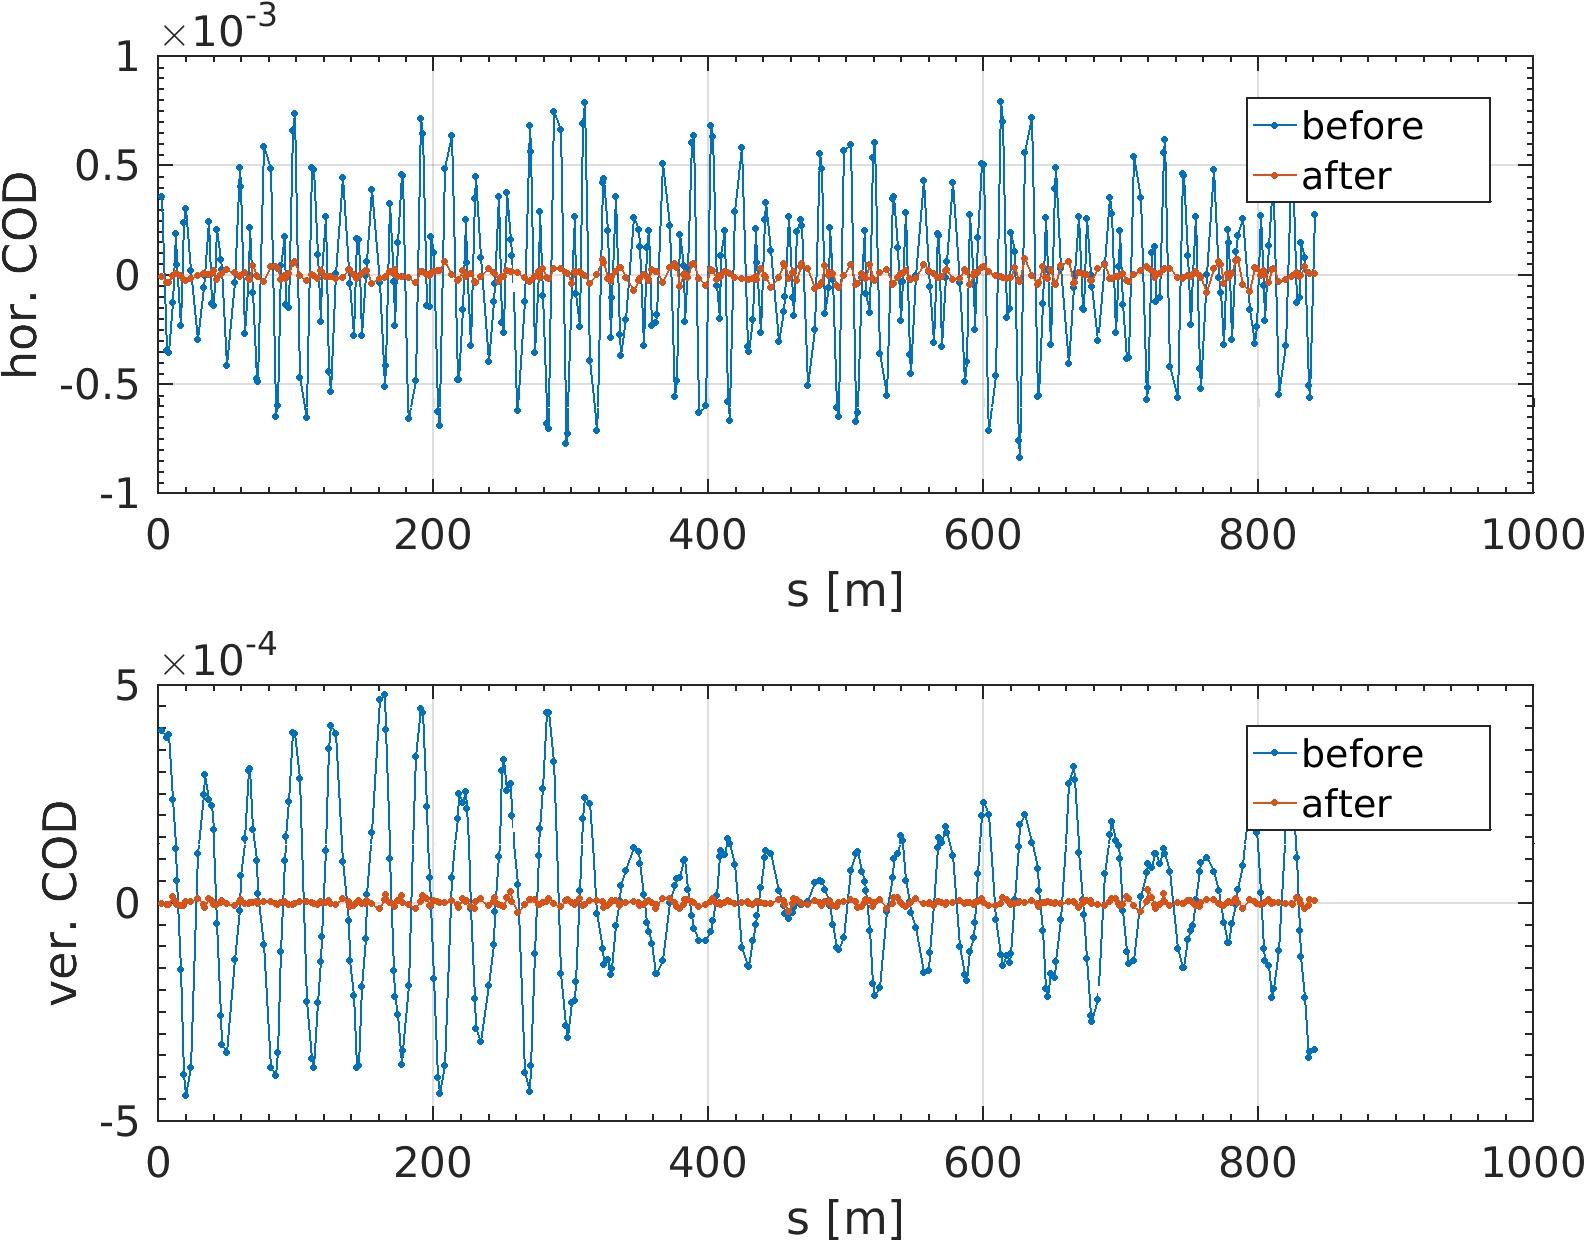
\includegraphics[width=0.98\textwidth]{./images/corrections/OrbitCor.jpg}
	\caption{Orbit correction using \emph{atcorrectorbit}}
	\label{fig:orbitcor}
\end{figure}


\clearpage
\subsubsection{Closed orbit bumps}
By giving a different orbit reference to \emph{atcorrectorbit}, it is possible to obtain closed orbit bumps. 
Below the code to obtain this result and a figure representing the result (figure \ref{})
\begin{lstlisting}
refx=zeros(size(indBPM));
refy=zeros(size(indBPM));

refx([7 8])=1e-4; % horizontal bump in position
refy([7 8])=[1e-4 -1e-4];  % vertical bump in angle

% correct restrictig response matrices
selbpm=[2  3    7 8   12 13]; % 6 and 9 missing, inside bump
selcor=[2  3           4  5]; % correctors

[rbump,...  			% lattice with COD bump
inCOD...
]=atcorrectorbit(...
    ring,...
    indBPM(selbpm),...
    indHCor(selcor),...
    indVCor(selcor),...
    inCOD,...
    repmat([4 4],3,1),... % iterate 3 times with 4 eigenvectors (all)
    [false false],...
    1.0,...
    [],... % compute RM for subset of bpm and correctors
    [refx(selbpm);...
     refy(selbpm)],...
    [],...
    true);
		
\end{lstlisting}

\begin{figure}[!h]
	\centering
	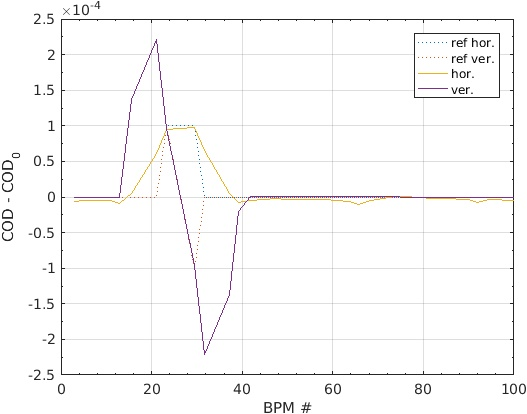
\includegraphics[width=0.5\textwidth]{./images/corrections/CODbump.jpg}
	\caption{Orbit bump in hor. plane and angle bump in ver. plane using \emph{atcorrectorbit}}
	\label{fig:orbitbump}
\end{figure}

\newpage
\subsection{Dispersion}

Dispersion correction is performed using \emph{atcorrectdispersion}. The functions implements several features for correction:
\begin{itemize}
\item the average correctors strenghts 0, 
\item iteration of the correction varying the number of eigenvectors 
\item correction of the frequency (dpp/quadrupoles response).
\item possibility to limit the correctors strengths
\end{itemize}

Below an example of usage of the orbit correction function. 
\begin{lstlisting}
% initial closed orbit guess and dispersion
inCOD=[0 0 0 0 0 0]';
[l,~,~]=atlinopt(ring,0,indBPM);
refdispersion=zeros(2,length(indBPM));
refdispersion(1,:)=arrayfun(@(a)a.Dispersion(1),l);
refdispersion(2,:)=arrayfun(@(a)a.Dispersion(3),l);


[rcor,...
inCOD,...
hs,vs...   				% total quadrupole strengths after correction
]=atcorrectdispersion(...
    rerr,... 			% lattice with errors to correct
    indBPM,...		% BPM indexes
    indQCor,...	 	% quadrupole correctors indexes
    indSCor,...		% skew quad. correctors indexes	
    inCOD,...			% initial COD guess 6D
    [floor(linspace(20,250,7));...   % eigenvectors at each iteration
     floor(linspace(20,250,7))]',...
    [false true],... % [correct DPP, keep average correctors zero]
    1.0,...				% scale factor for correction
    ModelRM,...		% model RM, if  [], compute it
    refdispersion,... % model dispersion
    [],...				% correctors limits, default= no limits 
    true); 				% verbosity

\end{lstlisting}

\begin{figure}[!h]
	\centering
	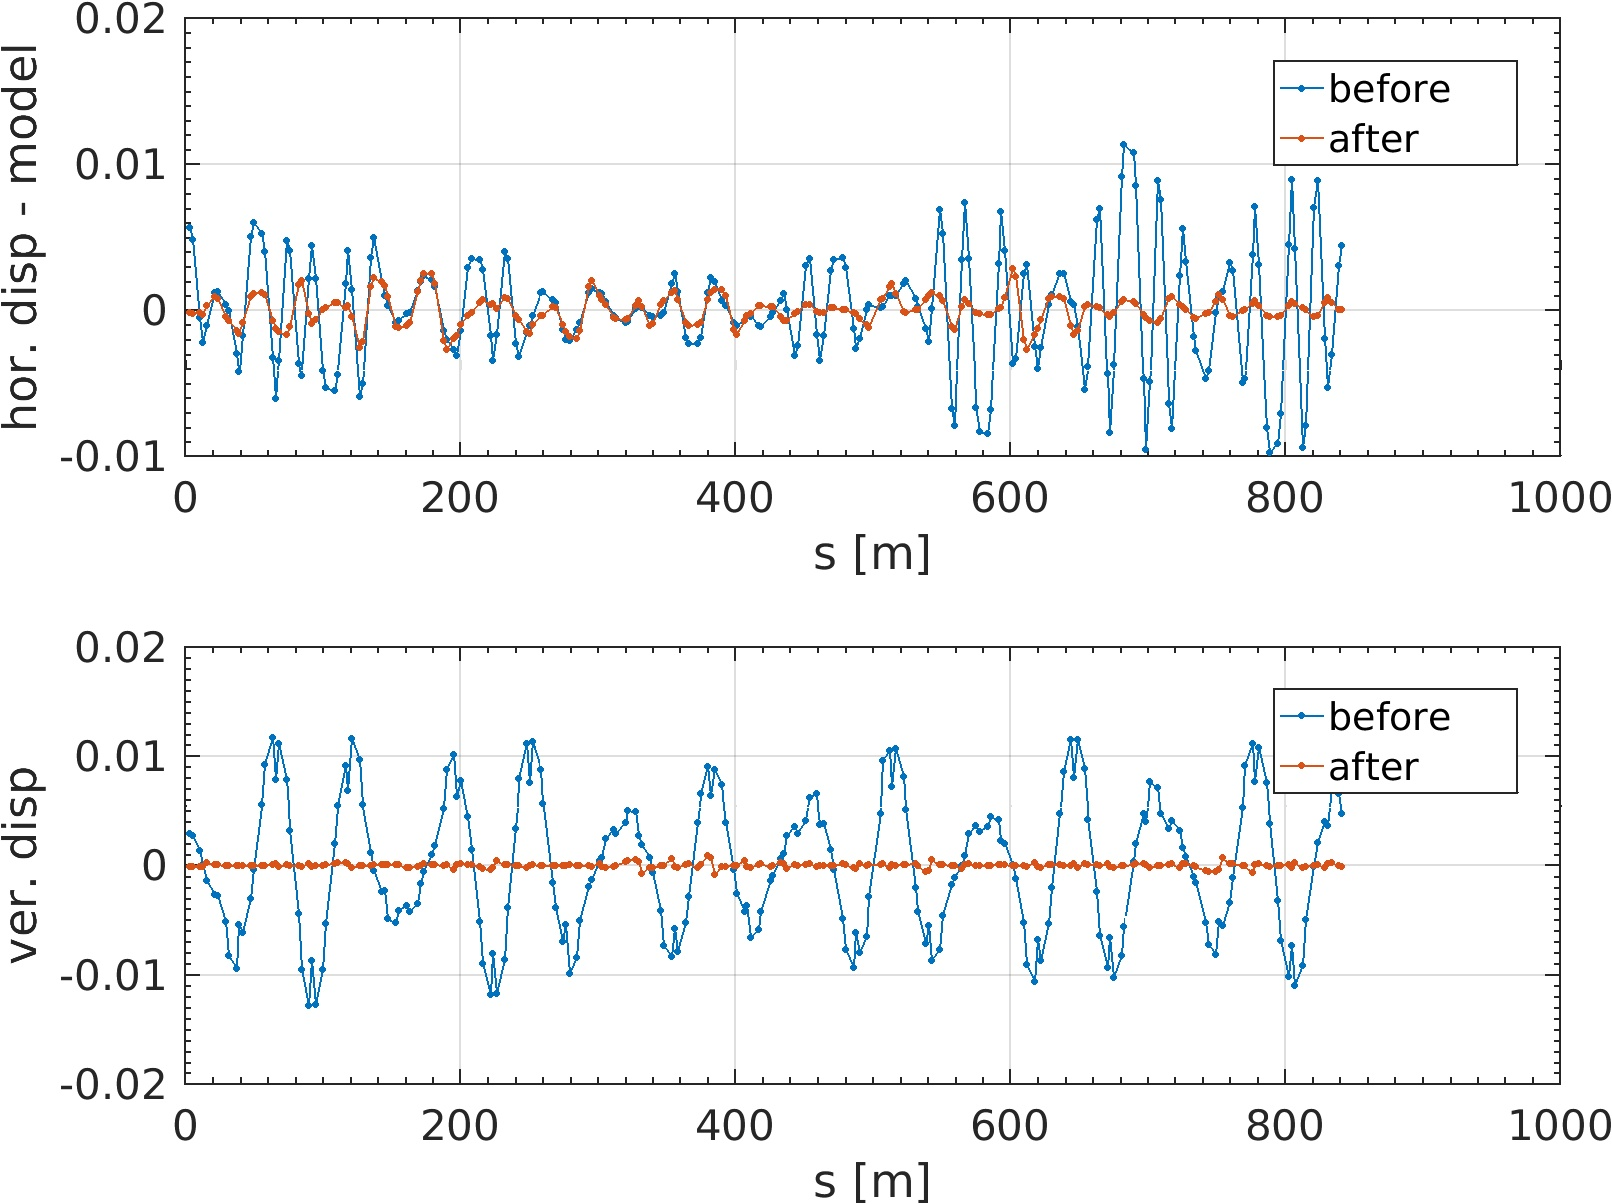
\includegraphics[width=0.98\textwidth]{./images/corrections/DispCor.jpg}
	\caption{Dispersion correction using \emph{atcorrectdispersion}}
	\label{fig:orbitcor}
\end{figure}

\clearpage
\subsection{Dispersion free steering}
The function \emph{atdispersiofreesteering} uses the steerers to simultaneously correct orbit and dispersion (dispersion free steering \cite{DFS}. The function implementation is very similar to the one of orbit and dispersion correction, but adds a weight parameter to tue the relative correction of orbit and dispersion.

\begin{lstlisting}
% same input as atcorrectorbit, apart for indicated
[rcor,inCOD,hs,vs]=atdispersionfreesteering(...
    rerr,...
    indBPM,...
    indHCor,...
    indVCor,...
    inCOD,...
    [floor(linspace(20,96,7));...   % eigenvectors at each iteration
     floor(linspace(20,97,7))]',...
    [true false],...
    1.0,...
    0.9,...   % <-- dispersion weigth
    ModelRM,...
    zeros(2,length(indBPM)),...
    refdispersion,...  % <-- dispersion reference
    [],...
    true);
		\end{lstlisting}

\begin{figure}[!h]
	\centering
	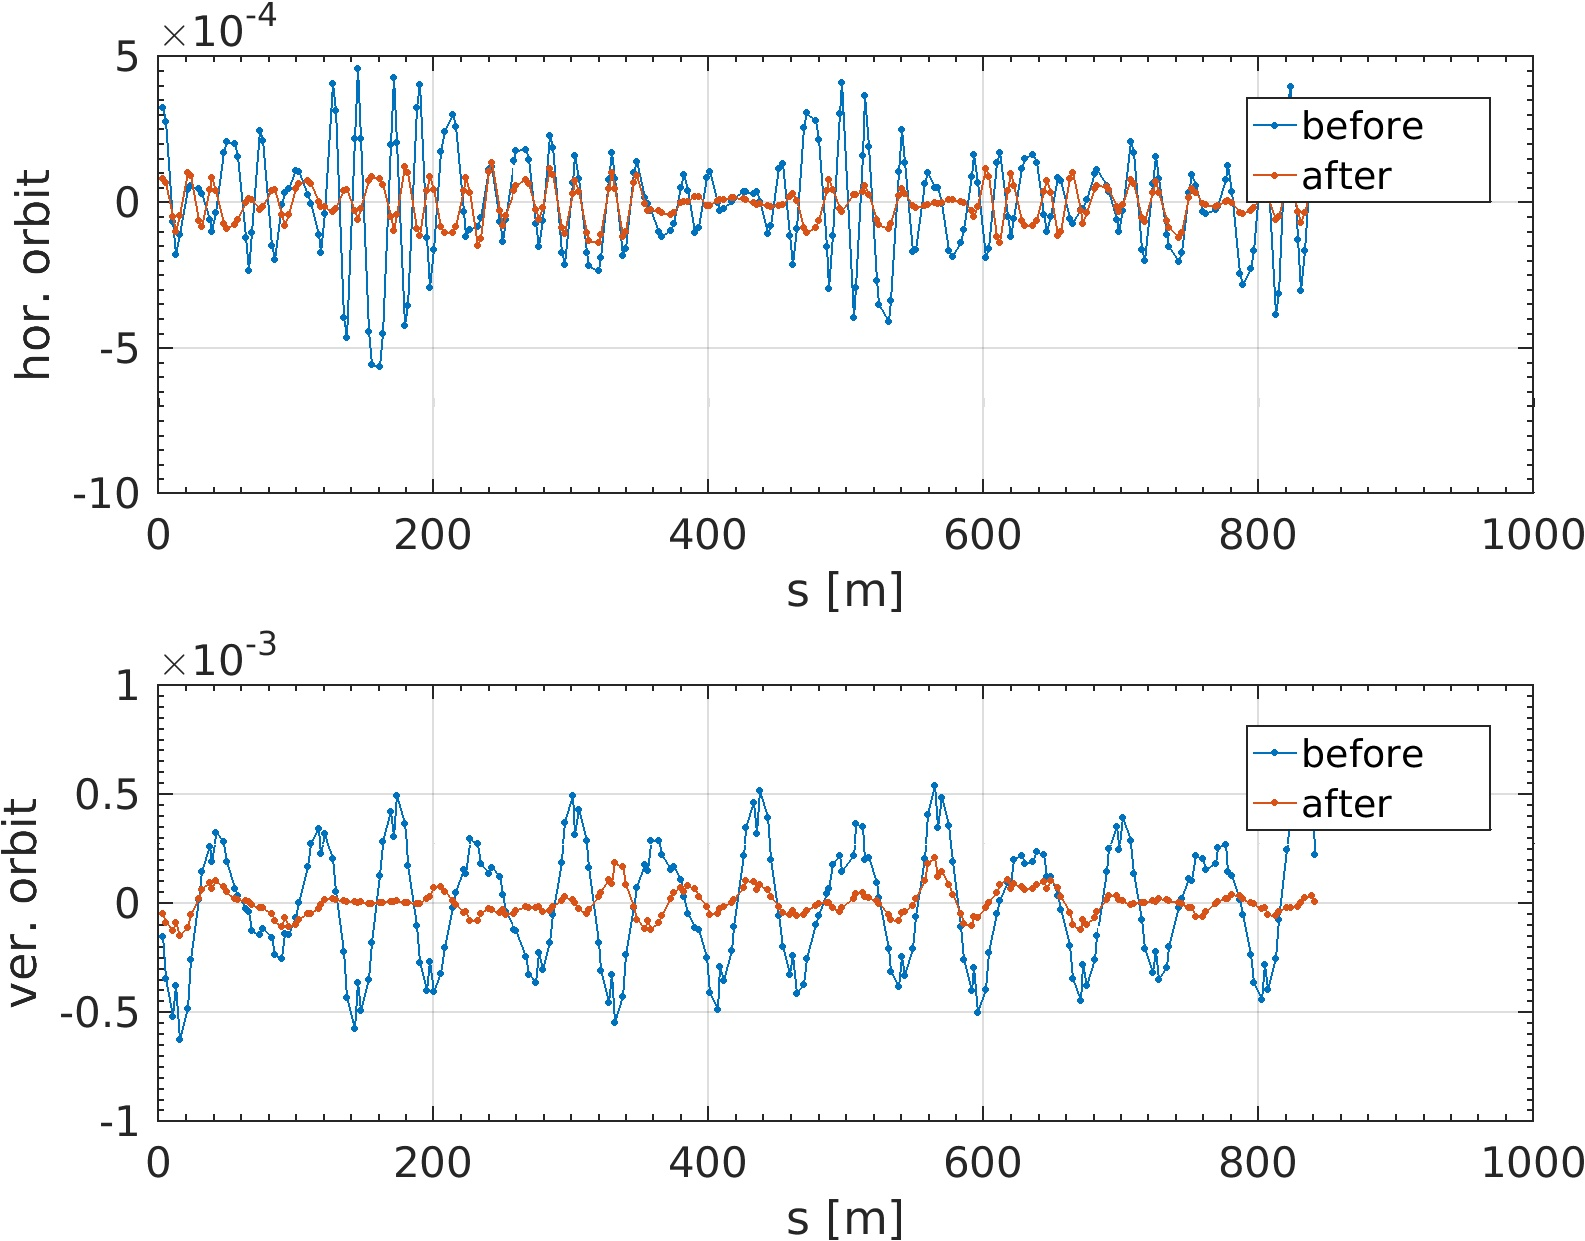
\includegraphics[width=0.45\textwidth]{./images/corrections/DFS/OrbCor.jpg}
	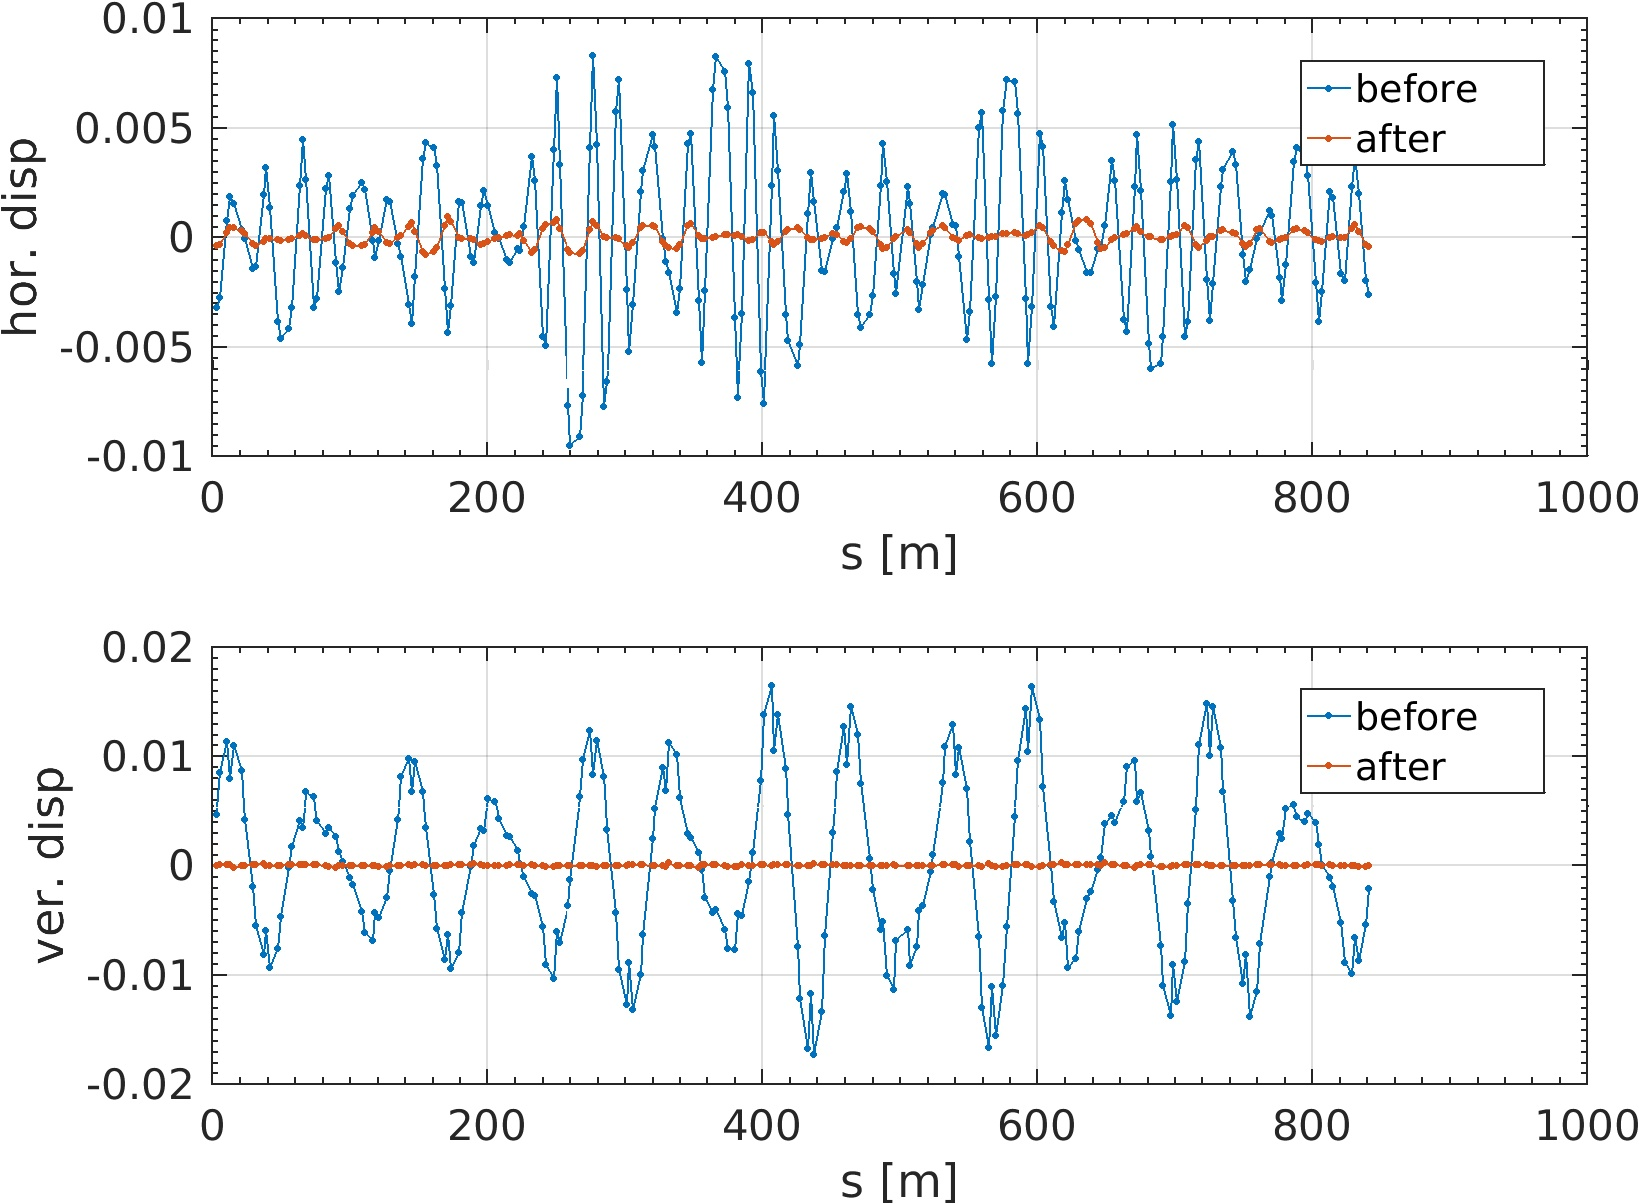
\includegraphics[width=0.45\textwidth]{./images/corrections/DFS/DispCor.jpg}\\
	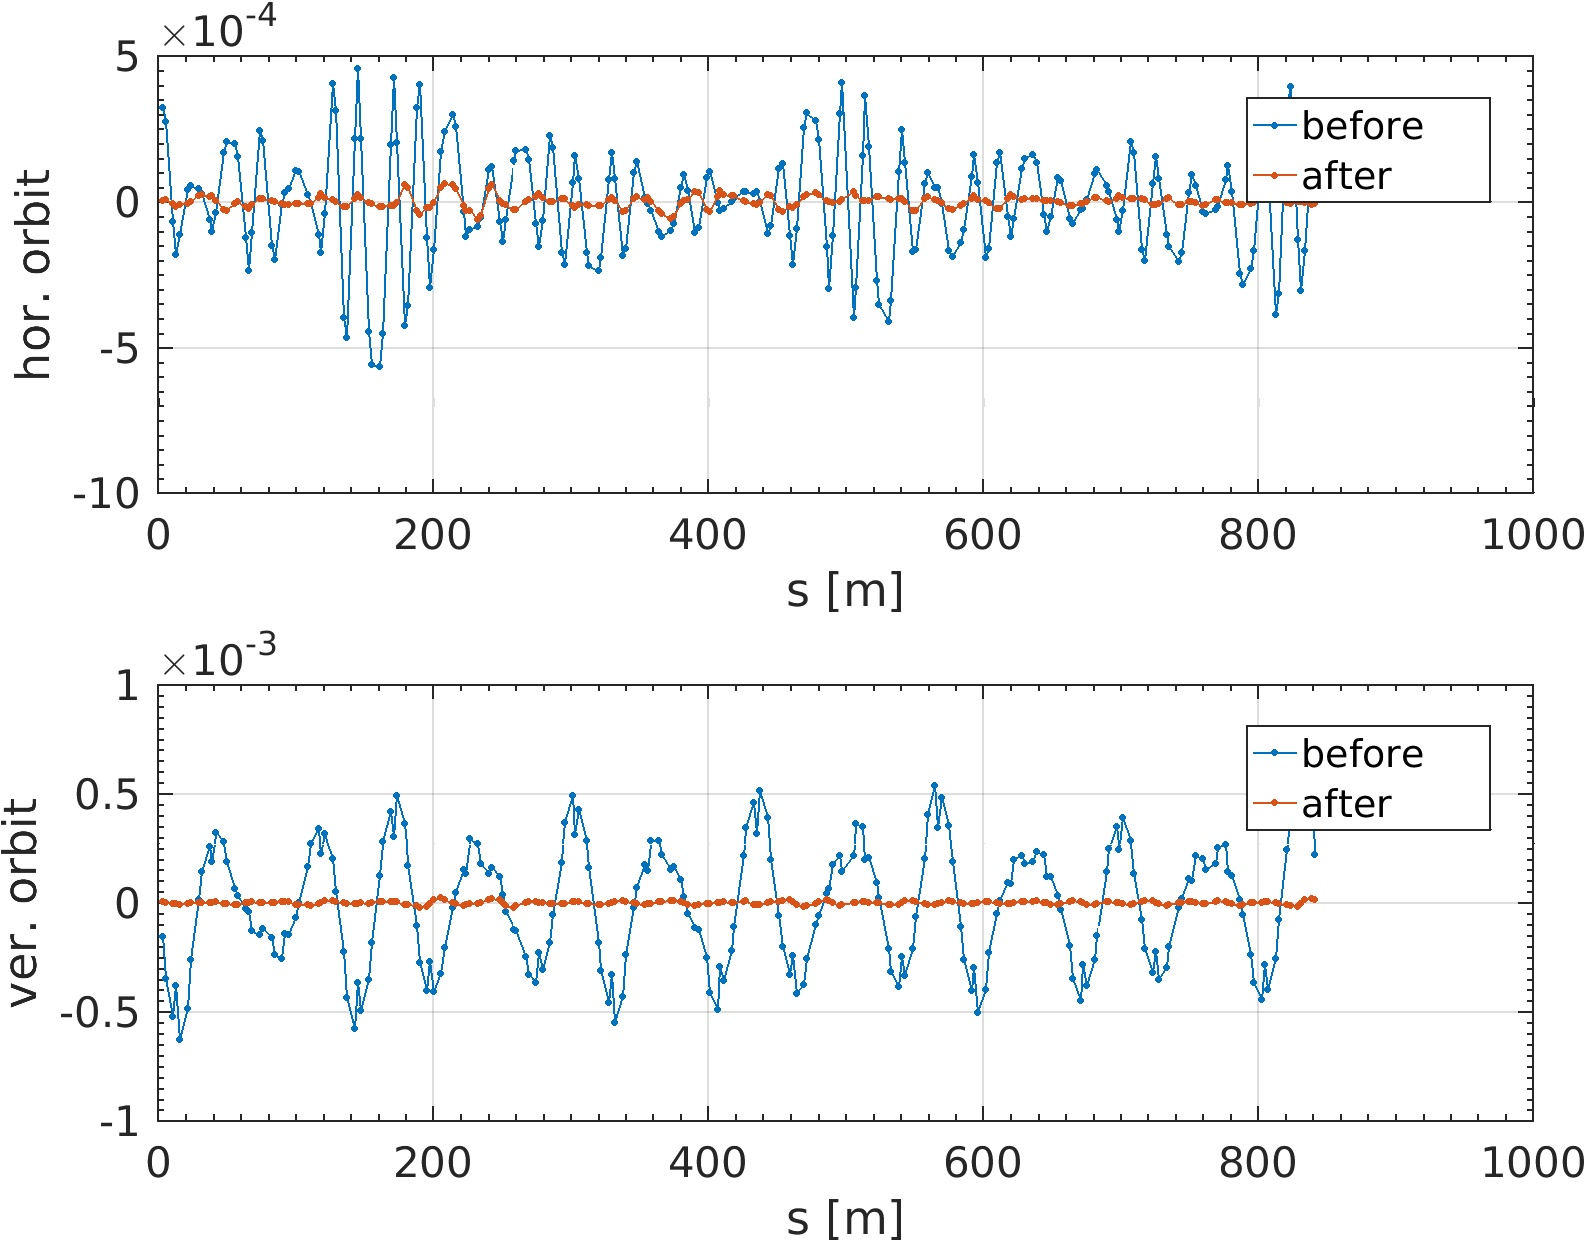
\includegraphics[width=0.45\textwidth]{./images/corrections/DFS/OrbCorNoDisp.jpg}
	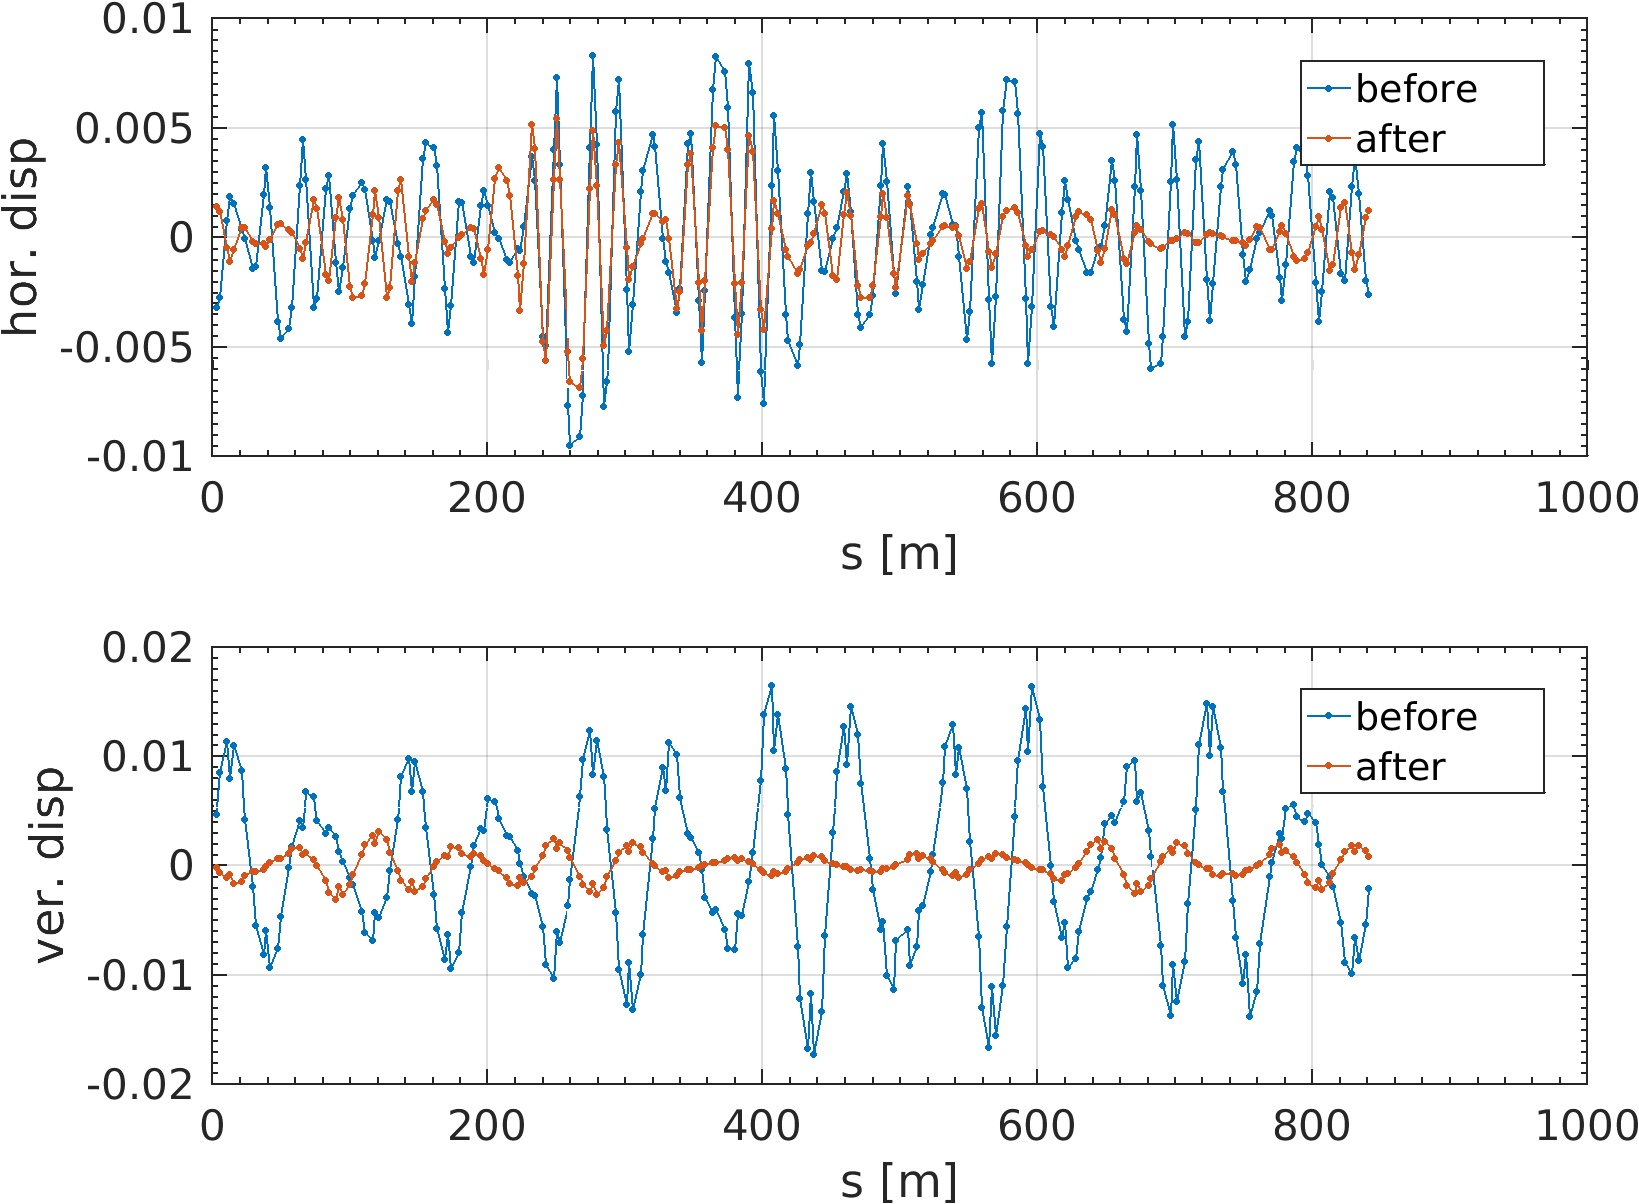
\includegraphics[width=0.45\textwidth]{./images/corrections/DFS/DispCorNoDisp.jpg}
	\caption{Dispersion free steering using \emph{atdispersiofreesteering}. Top plots, include the dispersion in the correction, bottom ones correct only orbit (weigth = 0.0) }
	\label{fig:DFScor}
\end{figure}

\subsection{Correction of RDT}
The correction of optics may be performed inverting a response to beta functions or phase advance. Unfortunately these parameters do not depend linearly on the normal and skew quadrupoles strengths. In \cite{RDTAndrea} we find a solution to this problem: the correction of normal and skew quadrupole resonance driving terms (RDT). This kind of correction is perfectly suited for the correction of a fitted lattice model that includes normal and skew quadrupoles errors. The functions retrieves the normal and skew quadrupole components in the lattice and computes the RDT values. Then the real and imaginary part of those terms are corrected in a system with dispersion and tunes. This correction is implemented in the function \emph{atRDTdispersioncorrection}. Three spin-off functions are also present:
\begin{itemize}
\item \emph{atRDTdispersioncorrection}: normal and skew quadrupole RDT, dispersion and tune correction
\item \emph{atQuadRDTdispersioncorrection}: normal quadrupole RDT, dispersion and tune correction
\item \emph{atSkewRDTdispersioncorrection}: skew quadrupole RDT, dispersion and tune correction
\item \emph{atRDTdispersionmeasuredcorrection}: normal and skew quadrupole RDT, measured dispersion and tune correction
\end{itemize}
An example of the application of the correction is shown below and in figure \ref{fig:RDTcor0p8} and \ref{fig:RDTcor0}.

\begin{lstlisting}

[rcor,...				% corrected lattice
inCOD,...
hs,...					% total quadrupole strengths
vs...						% total skew quadrupole strengths
]=atRDTdispersioncorrection(...
    rerr,...			% lattice with errors, or better, fitted errors model from RM measurements
    r0,...				% reference lattice to compute RDT and dispersion
    indBPM,...
    indQCor,...
    indSCor,...
    inCOD,...
    [...          % number of eigenvector at each iteration for 
    [15 30];...		% quad and skew quad correctors
    [30 60];...
    ],...
    [true],...    % average correctors to zero
    1.0,... 			% scale factor
    [0.8 0.1 0.8],...		% weigths for hor. dispersion, tune, ver. dispersion
    ModelRM);			% Response matrices, if[], compute them.
		
\end{lstlisting}

\begin{figure}[!h]
	\centering
	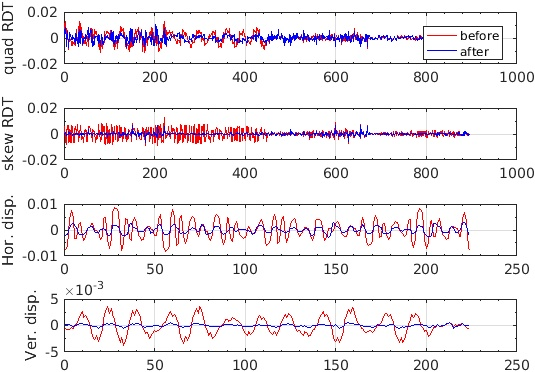
\includegraphics[width=0.95\textwidth]{./images/corrections/RDT/RDTdispCor0p80_0p10_0p80_.jpg}
	\caption{RDT and Dispersion correction using \emph{atRDTdispersiocorrection}. Dispersion weigth = 0.8 }
	\label{fig:RDTcor0p8}
\end{figure}

\begin{figure}[!h]
	\centering
	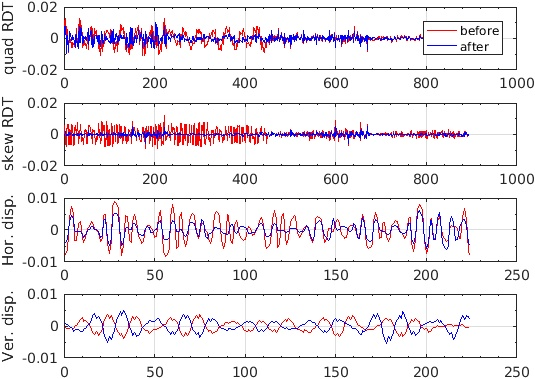
\includegraphics[width=0.95\textwidth]{./images/corrections/RDT/RDTdispCor0p00_0p00_0p00_.jpg}
	\caption{RDT and Dispersion correction using \emph{atRDTdispersiocorrection}. Dispersion weigth = 0.0 }
	\label{fig:RDTcor0}
\end{figure}

\subsection{Coupling free steering}
\subsubsection*{description}
\subsubsection*{example}
\begin{lstlisting}
% matlab code here
\end{lstlisting}

\subsection{Open trajectory correction}
If the errors set in the lattice are too large, it is possible that no COD is found by AT. This problem is often found in real commisioning, when the first turn is not at all granted. The function \emph{atfirstturntrajectory} finds a first turns COD by using the available trajectory at BPMs. 

The algorithm follows these steps:
\begin{itemize}
\item look for all BPMs with signal below a given threshold and correct the trajectory using a response computed from the model without errors. 
\item if all BPM see a signal, close the trajectory using the last 2 correctors in the lattice to match the reading of the first 2 BPMs.
\item if stack at less then all the BPMs, then increase the threshold up to +1mm
\item if still stack, look for an optimal injection point.
\item if still failing to get to the end of the lattice, compute trajectory response on lattice with errors. 
\end{itemize}
The number of correctors used can be limited to a  

\begin{lstlisting}
inCOD=[0 0 0 0 0 0]';

[rcor,...							% lattice with COD
inCOD...  						% intial orbit guess
]=atfirstturntrajectory(...
    rerr,...					% lattice without COD
    inCOD,...					% initial COD guess
    indBPM,...				% bpm indexes
    indHCor,...				% hor. steerers indexes
    indVCor,...				% ver. steerers indexes
    0.5e-2,...				% bpm reading limit [m]
    30,...						% corrector to use beofre last BPM with signal
    [false true],...	% [dpp correction, average correctors to zero]	
    ModelRM,...				% RM, if[], compute
    zeros(2,length(indBPM)),...	% reference orbit
    [],...						% steerers strengths limits
		true);						% verbosity	
		
\end{lstlisting}


\begin{figure}[!h]
	\centering
	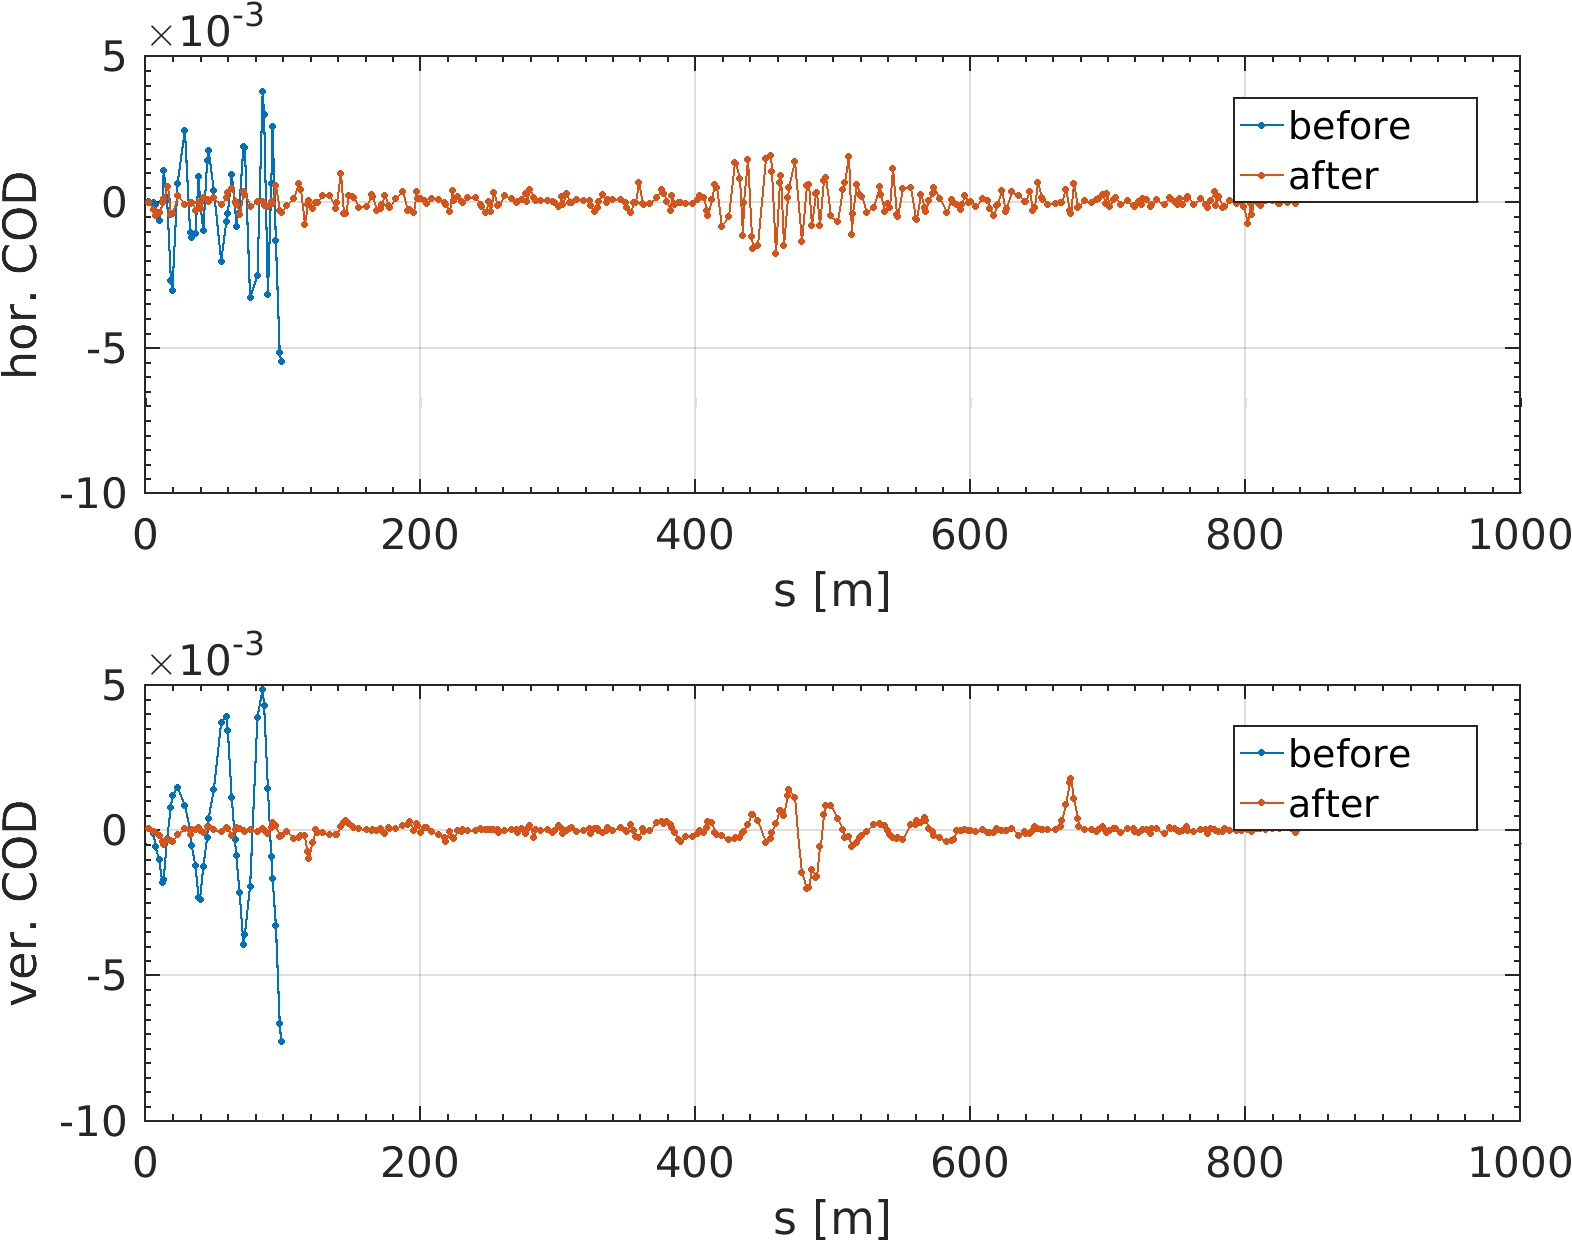
\includegraphics[width=0.95\textwidth]{./images/corrections/TrajCor.jpg}
	\caption{Trajectory correction using \emph{atfirstturntrajectory}. }
	\label{fig:trajcor}
\end{figure}


\subsection{Commissioning like correction sequence}
The above correction are often requested in a sequence. The function \emph{CorrectionChain} allows to perform a full correction sequence calling the above functions from a single entry point. 

\begin{lstlisting}
neigenvectors=[...
    200,... % n eig orbit H
    200,... % n eig orbit V
    200,... % skew quadrupole 
    250,... % normal quadrupole 
    350,... % fit normal quadrupole 
    100,... % fit dipole 
    350,... % fit skew quadrupole 
    ]; % number of eigenvectors 

cororder=[0 1 2 3 7 1 2 3 7 1 2 3 -1];
%  '(-1 ): RF cavity frequency and time lag tuning '...
%  '( 0 ): open trajectory (finds closed orbit) '...
%  '( 1 ): orbit '...
%  '( 2 ): tune '...
%  '( 3 ): chromaticity '...
%  '( 4 ): dispersion '...
%  '( 5 ): dispersion free steering '...
%  '( 6 ): rdt + dispersion correction '...
%  '( 7 ): fit errors model and correct model quad RDT + dispersion (6)'

speclab='test';
verbose=true;

[...
    rcor,...            % corrected lattice
		ch,...              % final H cor values
    cv,...              % final V cor values
    cq,...              % final Quad cor values
    cs...               % final Skew Quad cor values
    ]=CorrectionChain(...
    rerr,...            %1  initial lattice with errors
    r0,...              %2  model lattice
    indBPM,...          %3  bpm index
    indHCor,...         %4  h steerers index
    indVCor,...         %5  v steerers index
    indSkewQuadCor,...  %6  skew quad index
    indQuadCor,...      %7  quadrupole correctors index
    Neig,...            %8  number of eigen vectors [NeigorbitH, NeigorbitV,   NeigQuadrdt, Neigdispv, Neigdisph,neig rdt corr, SkewQuadRDT]
    corrorder,...       %9  correction order 1: orbit, 2: tune, 3: skewquad disp v 4: quad disp h 5: quad RDT 6: skew RDT
    ModelRM,...          %10 response matrices
    speclab,...          %11 response matrices
    verbose)             %12 verbose (false): if true print out all relevat quantities after each step in corrorder



\end{lstlisting}

\newpage
